\documentclass{article}
\usepackage[english]{babel}
\usepackage[utf8]{inputenc}
\usepackage{fancyhdr}
\usepackage{amsmath}
\usepackage{amsfonts}
\usepackage{mathrsfs}
\usepackage{mathtools}
\usepackage{indentfirst}
\usepackage{hyperref}
\usepackage{tikz,amsmath}
\usepackage{tikz,tkz-tab,amsmath}
\usetikzlibrary{trees}
\usetikzlibrary{arrows}
\usepackage{enumerate}

%\setlength{\TPHorizModule}{1mm}
%\setlength{\TPVertModule}{1mm}
  
\hypersetup{
    colorlinks=true,
    linkcolor=blue,
    filecolor=magenta,
    urlcolor=blue,
}
\urlstyle{same}

\parskip 1ex

\usepackage{geometry}
 \geometry{
 a4paper,
 left=20mm,
 top=20mm,
 bottom=20mm,
 right=20mm
 }
\usepackage{multicol}
\pagestyle{fancy}
\fancyhf{}
\lhead{Matthieu Bessat}
\rhead{DM 2}
\rfoot{Page \thepage}

\makeatletter
\def\@seccntformat#1{%
  \expandafter\ifx\csname c@#1\endcsname\c@section\else
  \csname the#1\endcsname\quad
  \fi}
\makeatother

\newcommand{\vspacem}{\vspace{2mm}}
\newcommand{\bfrac}[2]{\displaystyle\frac{#1}{#2}}
\newcommand{\bbinom}[2]{\displaystyle\binom{#1}{#2}}

\newif\ifquoteopen
\catcode`\"=\active % lets you define `"` as a macro
\DeclareRobustCommand*{"}{%
   \ifquoteopen
     \quoteopenfalse ''%
   \else
     \quoteopentrue ``%
   \fi
}

\begin{document}

\subsection*{Exercice 1}

\textbf{1.} $\mathcal{D}_f = \mathbb{R}_+^* = ]0, +\infty[$
\vspacem
% \renewcommand{\theenumi}{(\roman{enumi})}%
% \begin{enumerate}
%   \item $\bbinom{10}{3} = 120$
%   \item $\bbinom{10}{4} = 210$
%   \item $\bbinom{10}{4} = 210$
%   \item $\bbinom{10}{5} = 252$
% \end{enumerate}

%\noindent 

\noindent $f$ est dérivable sur $R_+^*$ : \quad $f'(x) = x^x (\ln(x) +1)$

\noindent On sait que $\forall x \in \mathbb{R_+^*}, \; x^x > 0$. Donc le signe de $f'(x)$ dépend de $(\ln(x) + 1)$ :

$\ln(x) + 1 > 0 \Leftrightarrow \ln(x) > -1 \Leftrightarrow x > e^{-1}$

\begin{align*}
x^x &\xrightarrow[x \to 0]{} 1           &     x^x &\xrightarrow[x \to +\infty]{} +\infty
\end{align*}

\begin{center}
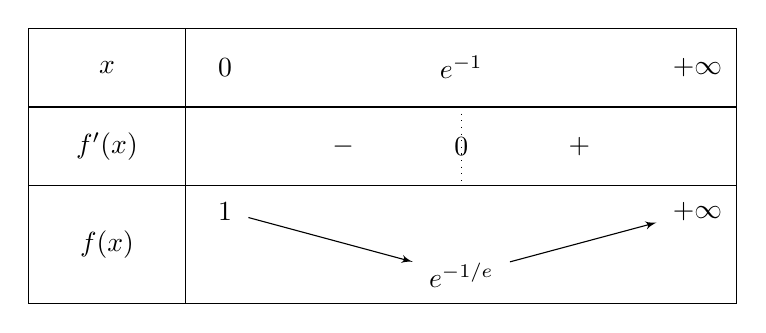
\begin{tikzpicture}
\tkzTabInit[]{
    $x$ /1,
    $f'(x)$ /1,
    $f(x)$ /1.5
}{
    $0$,
    $e^{-1}$,
    $+\infty$
}
\tkzTabLine{,-,z,+,}
\tkzTabVar{+/$1$,-/$e^{-1/e}$,+/$+\infty$}
\end{tikzpicture}
\end{center}

\noindent Avec $f(e^{-1}) = e^{-1/e} \approx 0.69$ 

\vspacem
\textbf{2.} On pose $h(x) = x\ln(x) - \ln(x) = \ln(x)(x - 1)$
\vspacem

\begin{center}
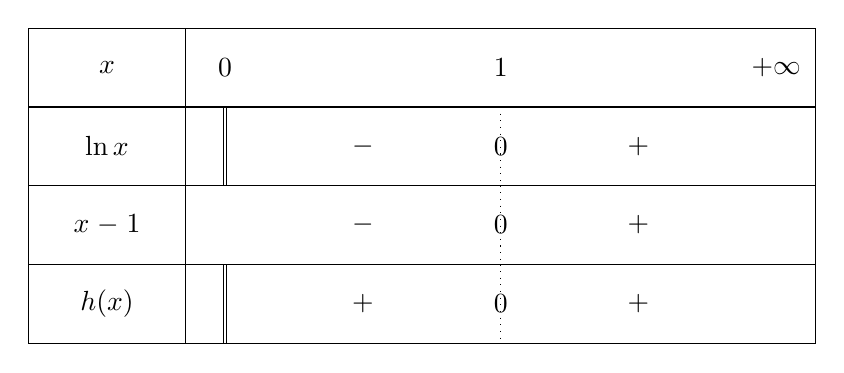
\begin{tikzpicture}
\tkzTabInit[lgt=2, espcl=3.5]{
    $x$ /1,
    $\ln x$ /1,
    $x-1$ /1,
    $h(x)$ /1
}{
    $0$,
    $1$,
    $+\infty$
}
\tkzTabLine{d,-,z,+}
\tkzTabLine{,-,z,+}
\tkzTabLine{d,+,z,+}
\end{tikzpicture}
\end{center}

% \noindent On calcule $h'(x)$ :

% $h'(x) = (\ln(x))'(x-1) + (x-1)'\ln(x) = \bfrac{x-1}{x} + \ln(x) = 1 - \bfrac{1}{x} + \ln(x)$

\noindent On a donc $\forall x \in \mathbb{R}^*_+$, $h(x) \geq 0$

\noindent Ainsi, $\forall x \in \mathbb{R}^*_+$, $\ln(x) \leq x \ln (x)$

\vspacem
\textbf{3.}
\begin{flalign*}
\Delta : \quad &y = f(1) + f'(1)(x-1) &&\\
&y = 1^1 + 1^1(\ln(1)+1)(x-1) &&\\
&y = 1 + (x-1) = 1 + x - 1 = x
\end{flalign*}
\noindent Pour étudier la position relative de $\Delta$ et $\mathcal{C}$ on étudie le signe de $g(x)$ :

$g(x) = f(x) - x = x^x - x$

$g'(x) = x^x(\ln x + 1) -1$
\begin{flalign*}
(*) &\Leftrightarrow g'(x) \geq 0 &&\\
&\Leftrightarrow x^x(\ln(x) + 1) -1 \geq 0 &&\\
&\Leftrightarrow x^x(\ln(x) +1) \geq 1 &&\\
&\Leftrightarrow \ln(x) +1 \geq 1 \quad &&\\
%\text{(Car }\forall x \in \mathbb{R}_{+}^{*}, \; x^x > 0\text{)} &&\\
&\Leftrightarrow \ln(x) \geq 0 &&\\
&\Leftrightarrow x \geq 1
\end{flalign*}

$g(1) = f(1) - 1 = 1^1 - 1  = 0$

\noindent On en déduit le tableau de variation suivant :

\vspacem
\begin{center}
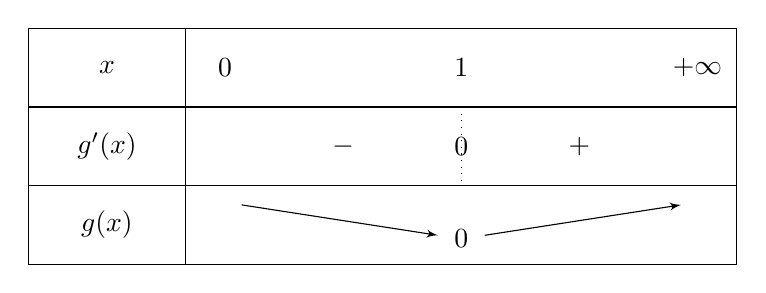
\begin{tikzpicture}
\tkzTabInit[]{
    $x$ /1,
    $g'(x)$ /1,
    $g(x)$ /1
}{
    $0$,
    $1$,
    $+\infty$
}
\tkzTabLine{,-,z,+,}
\tkzTabVar{+/,-/$0$,+/}
\end{tikzpicture}
\end{center}

\noindent D'après le tableau de variation, $\forall x \in \mathbb{R}_+^*, f(x) \geq x$

\noindent Donc $\mathcal{C}$ est soit au-dessus, soit confondu avec $\Delta$. $\Delta$ est une tangente de $\mathcal{C}$, une courbe convexe.

\vspacem
\textbf{4.} D'après le tableau de variation décrit à la question 1. et puisque $f$ est strictement monotone et continue sur l'intervalle $I$. On a $f$ qui définit une bijection de I sur J :

% \, \longrightarrow \, [e^{-1/e}, +\infty[$

\noindent La bijection réciproque $\varphi$ est la fonction réciproque de $f(x)$ qui à $J = [e^{-1/e}, +\infty[$ associe $I = [e^{-1}, +\infty[$.

\noindent Vu que $\varphi$ est une bijection, elle est continue et monotone sur $[e^{-1/e}, +\infty[$

\vspacem
\textbf{5.}
\vspacem
%\noindent $\forall y \in I$, montrons que :
\noindent Soit $y \in J$, on a : $y = f(\varphi(y))$
\begin{flalign*}
&\quad \varphi(y)^{\varphi(y)} = y &&\\
&\Leftrightarrow \ln(\varphi(y)^{\varphi{y}}) = \ln(y) &&\\
&\Leftrightarrow \varphi(y) \ln(\varphi(y)) = \ln(y) &&\\
&\Leftrightarrow \ln(\varphi(y)) = \bfrac{\ln(y)}{\varphi(y)}
\end{flalign*}

\textbf{6.}
\vspacem

\noindent On considère : $\bfrac{\varphi(y)}{\ln(y)} = \bfrac{1}{\ln(\varphi(y)}$

\noindent Aussi : $\displaystyle\lim_{y\rightarrow+\infty} \varphi(y) = +\infty$ car c'est la fonction réciproque de $\varphi$.

\[
\begin{matrix*}[r]
\left.\begin{matrix*}[r]    
   \displaystyle\lim_{y\rightarrow+\infty} 1 = 1\\
   \\
   \\
    \left.\begin{matrix*}
        \displaystyle\lim_{y\rightarrow+\infty} \varphi(y) = +\infty\\
       \\
       \displaystyle\lim_{Y\rightarrow+\infty} \ln(Y) = +\infty\\
    \end{matrix*}\medspace\right\}
    \left.\begin{matrix*}
        \space\text{par composée :}
        \vspace{2mm}\\
        \displaystyle\lim_{y\rightarrow+\infty} \ln(\varphi(y)) = +\infty
    \end{matrix*}\right.
\end{matrix*}\medspace\right\}
\left.\begin{matrix*}
    \space\text{par quotient :}\vspace{2mm}\\
    \displaystyle\lim_{y\rightarrow+\infty} \bfrac{1}{\ln(\varphi(y))} = 0
\end{matrix*}\right.
\end{matrix*}
\]

\noindent Donc on a bien :

\[
    \bfrac{\varphi(y)}{\ln(y)} \xrightarrow[y \to +\infty]{} 0
\]

\textbf{7.}

%\noindent $\varphi$ est dérivable sur l'intervalle $K = $
\newpage
\begin{flalign*}
\varphi(y) &= \bfrac{\ln(y)}{\ln(\varphi(y))} &&\\
\varphi'(y) &= \bfrac{
(\ln(y))' \ln(\varphi(y)) - (\ln(\varphi(y)))' \ln(y)
}{\ln(\varphi(y))^2} &&\\
\varphi'(y) &= \bfrac{\frac{\ln(\varphi(y))}{y} - \frac{\varphi'(y)}{\varphi(y)}\ln(y)}{\ln(\varphi(y))^2} &&\\
\varphi'(y) &= \bfrac{\frac{\ln(\varphi(y))}{y} - \varphi'(y) \ln(\varphi(y))}{\ln(\varphi(y))^2} &&\\
\varphi'(y) &= \bfrac{\ln(\varphi(y))\Big(\frac{1}{y} - \varphi'(y)\Big)}{\ln(\varphi(y))^2} &&\\
\varphi'(y) &= \bfrac{\frac{1}{y} - \varphi'(y)}{\ln(\varphi(y))} &&\\
\varphi'(y) + \bfrac{\varphi'(y)}{\ln(\varphi(y))} &= \bfrac{1}{y \times \ln(\varphi(y))} &&\\
\varphi'(y)\Big(1 + \frac{1}{\ln(\varphi(y))}\Big) &= \bfrac{1}{y \times \ln(\varphi(y))} &&\\
\varphi'(y) &= \bfrac{1}{y\ln(\varphi(y))} \times \bfrac{\ln(\varphi(y))}{\ln(\varphi(y)) + 1} &&\\
\varphi'(y) &= \bfrac{1}{y\Big(\frac{\ln(y) + \varphi(y)}{\varphi(y)}\Big)} &&\\
\varphi'(y) &= \bfrac{\varphi(y)}{y(\varphi(y) + \ln y)}
\end{flalign*}

\subsection*{Exercice 2}

%\setlength{\abovedisplayskip}{3pt}
%\setlength{\belowdisplayskip}{-1pt}

\textbf{8.}
\begin{flalign*}
(*) &\Leftrightarrow \arcsin(2x) - \arcsin(x\sqrt{3}) = \arcsin(x) &&\\
&\Leftrightarrow \sin(\arcsin2x - \arcsin(x\sqrt{3})) = x &&\\
&\Leftrightarrow \sin(\arcsin2x)\cos(\arcsin(x\sqrt3)) - \cos(\arcsin2x)\sin(\arcsin(x\sqrt{3})) = x &&\\
&\Leftrightarrow 2x \times \cos(\arcsin x\sqrt{3}) - \cos(\arcsin 2x) \times x\sqrt{3} = x
\end{flalign*}
\noindent Or :
\begin{flalign*}
(\triangle) &\Leftrightarrow \cos^2x + \sin^2x = 1 &&\\
&\Leftrightarrow \cos^2x = 1 - \sin^2x &&\\
&\Leftrightarrow \cos x = \sqrt{1 - \sin^2x}
\end{flalign*}
\noindent Donc :
\begin{flalign*}
(*) &\Leftrightarrow 2x\sqrt{1 - \sin^2(\arcsin x\sqrt{3})} -  x\sqrt{3}\sqrt{1 - \sin^2(\arcsin 2x)} = x &&\\
&\Leftrightarrow 2x\sqrt{1 - (x\sqrt{3})^2} -  x\sqrt{3}\sqrt{1 - (2x)^2} = x &&\\
&\Leftrightarrow 2x\sqrt{1-3x^2} - x\sqrt{3}\sqrt{1 - 4x^2} = x &&\\
&\Leftrightarrow 2x\sqrt{1-3x^2} - x\sqrt{3 - 12x^2} = x&&\\
&\Leftrightarrow 2x\sqrt{1-3x^2} - x\sqrt{3 - 12x^2} - x = 0 &&\\
&\Leftrightarrow x \Big(2\sqrt{1-2x^2} - \sqrt{3-12x^2} - 1\Big) = 0 &&\\
\end{flalign*}
\noindent Une des solution à $(*)$ est donc 0.
\begin{flalign*}
(\Upsilon) &\Leftrightarrow 2\sqrt{1-3x^2} - \sqrt{3 - 12x^2} - 1 = 0 &\\
&\Leftrightarrow 4(1-3x^2) = (\sqrt{3-12x^2} + 1)^2 &\\
&\Leftrightarrow 4 - 12x^2 = 3 - 12x^2 + 2\sqrt{3-12x^2} + 1 &\\
&\Leftrightarrow 0 = 2\sqrt{3 - 12x^2}&\\
&\Leftrightarrow 0 = 4(3 - 12x^2)&\\
&\Leftrightarrow 0 = - 48x^2 + 12&\\
\end{flalign*}

\noindent Calcul du discriminant : 

$\Delta = b^2 - 4ac = 0 + 4\times 48 \times 12 = 2304$

$\sqrt{\Delta} = 48$

$x_1 = \bfrac{-b + \sqrt{\Delta}}{2a} = \bfrac{-48}{2\times-48} = \bfrac{1}{2}$

$x_2 = \bfrac{-b - \sqrt{\Delta}}{2a} = \bfrac{48}{2\times-48} = -\bfrac{1}{2}$

\noindent Ainsi $S_{*} = \Big\{-\bfrac{1}{2}, \, 0,\, \bfrac{1}{2}\Big\}$

\end{document}

